% Indicate the main file. Must go at the beginning of the file.
% !TEX root = ../main.tex

%----------------------------------------------------------------------------------------
% CHAPTER TEMPLATE
%----------------------------------------------------------------------------------------


\chapter{Hypothesengestützte Annäherung} % Main chapter title

\label{Chapter5} % Change X to a consecutive number; for referencing this chapter elsewhere, use \ref{ChapterX}

%----------------------------------------------------------------------------------------
% SECTION 1
%----------------------------------------------------------------------------------------
\section{Verwendungszusammenhänge statistischer Termini}
In Bezug auf die Fragestellung haben sich aus der induktiven, \textit{corpus-driven} Perspektive zunächst keine klaren Erkenntnisse herausgestellt. Ziel der Arbeit ist es ja, anhand des deutschschweizerischen Schuldiskurses im 19.~Jahrhundert aufzuzeigen, dass Statistik eine Funktion der «Digitialisierung» der Gesellschaft ist. Sie soll die zunehmende gesellschaftliche Komplexität der modernen, post-ständischen Gesellschaft handhabbar und beschreibbar machen. Diese Komplexität ist in der Schule besonders drängend, da sie in dieser Gesellschaft erstmals den theoretischen Anspruch erhebt, dass alle Staatsangehörigen ein gewisses Ausmass an standardisierter Volksschulbildung geniessen sollen. 

Die Korpusexploration hat zumindest den Nachweis erbracht, dass statistische Termini im Untersuchungskorpus signifikant vorkommen und dies besonders in der zweiten Hälfte, das heisst ab etwa den 1830er-Jahren. Davon ausgehend sollen einige Hinweise weiterverfolgt und mit Annahmen kombiniert werden, um die Fragestellung beantworten zu können. Im Sinne des Forschungsdesigns ist dies der zweite Strang einer hypothesengestützen Korpusanalyse.

\section{Was Statistiken zählen}

\subsection{Schülerinnen und Schüler}

Die grundlegende Operation der Statistik ist das Zählen, sei es die Zahl der Staatsangehörigen, Schüler*innen oder Diebstähle. Zählen ist aber nicht voraussetzungslos. Es braucht eine vorherige Definition dessen, was gezählt werden soll. Wie Hacking betont, braucht man zum Zählen Kategorien. Gezählt werden kann nur, was vorher als addierbar bestimmt wurde. Dafür müssen unter Umständen disparate Realitäten auf einen gemeinsamen Aspekt reduziert werden (\cite[280]{hacking_biopower_1982}). Tatsächlich sind die Kategorien historischer Statistiken hochgradig variabel und ihre Entwicklung gibt Aufschluss über die Statistikgeschichte, aber auch gesellschaftliche Konstruktionen dessen, was untersucht wird. Einmal geschaffene Kategorien konnten dabei wieder auf den Untersuchungsgegenstand zurückwirken. Vanderstraeten zeigt dies am Beispiel der Einteilung in berufstätige und nicht-berufstätige Personen. Dass Individuen und ihr Beschäftigungsstatus gezählt werden, empfinden wir als normal. Es ist aber die Folge statistischer Kategorisierungen, die institutionell verankert sind und auf individueller Ebene als gesellschaftliche Wirklichkeit akzeptiert werden (\cite{vanderstraeten_soziale_2006}).

Entsprechend bietet sich auch für diese Arbeit an, zu fragen, was im Korpus gezählt wird, wenn es um Schüler*innen geht. Dafür wurden alle Vorkommnisse von Zahlen gesucht, die von Begriffen angeführt oder gefolgt werden (Abbildung~\ref{figure:5-1}).\footnote{Die Idee für diese Abfrage stammt von Philipp Dreesen.} Die Peaks in den Jahren 1815 und 1819 erklären sich durch die geringen Mengen an Text, die für diese Jahre im Korpus vertreten sind. Daher sorgen hier schon wenige Treffer (21 bzw.~11) für eine vergleichsweise hohe relative Häufigkeit. Beide rühren jeweils von einem einzigen Text her, der für die Fragestellung hier nicht relevant ist. Während die Form mit vorangestellter Zahl eher in Fliesstexten auftaucht und auf separate oder textexterne Tabellen verweist, findet sich zweitere Form mit nachgestellter Zahl wiederholt in Auflistungen. 

    \begin{figure}
        \begin{tikzpicture}    
        \pgfplotstableread[col sep=comma]{./Data/abbildung-5-1-anzahl_schueler.csv}{\loadedtable}
        \begin{axis}[
            ybar,
            width=\linewidth,
            ymajorgrids=true,
            xlabel=Jahr,
            ylabel=Treffer per Mio.~Wörter,
            legend style={at={(xticklabel cs:.5)},anchor=north},% Legende abhänging von xticks positioniert
            x tick label style={rotate=90,anchor=east},
            xmin = 1799,
            xmax = 1871,
            height = 7cm,
            bar width=3pt,
            xtick pos = left,
            ytick pos = left,
            ymin = 0,
          ]
        \addplot[x=Jahr, y=Treffer per Mio. Wörter, color=zhawgray, fill]table{\loadedtable};
        \end{axis} 
        \end{tikzpicture}  
        \caption{Relative Häufigkeit für \texttt{([pos="CARD"]\-[lemma=".*schü\-ler\-|.*schü\-lerin|\-Kna\-be|\-Mäd\-chen|\-Tochter|\-Kind|\-Schüler|\-Schül\-erin|Bu\-be"])|([lemma\-=".*schü\-ler\-|.*schü\-lerin|\-Kna\-be|\-Mäd\-chen|\-Tochter|\-Kind|\-Schü\-ler|\-Schü\-ler\-in|Bu\-be"][pos= "CARD"])}}
        \label{figure:5-1} 
    \end{figure}

In den Ergebnissen zeigt sich, nach welchen Kategorien Schüler*innen und Schulen gezählt wurden. Die Schulstatistik des Kantons Bern für das Schuljahr 1838/39 beispielsweise, also zu Beginn des «avalanche of numbers», zählte die Volksschüler*innen nach Geschlecht sowie die unterschiedlichen Schularten (Abbildung~\ref{figure:5-2}). 

\begin{figure}[!ht]
    \centering
    \includegraphics[width=0.7\textwidth]{../Figures/ass-001_1840_006_349_358_e739.jpg}
    \caption{Schulstatistik des Kantons Bern 1838/39 aus~\cite[356]{noauthor_kanton_1840}.}
    \label{figure:5-2}
\end{figure}

Die Statistik macht so sichtbar, wie viele Primarschulen im Kanton bestanden und wie viele männliche und weibliche Schüler*innen diese besuchten. Darüber hinaus bestand offensichtlich ein Interesse an öffentlichen Gemeindeschulen und wie viele seit 1831, dem Erlassjahr einer neuen liberalen Kantonsverfassung, gegründet wurden. Sie verschaffte also den Diskursteilnehmer*innen einen Überblick über die Expansion der öffentlichen Primarschule, einem zentralen Anliegen der liberalen Bewegung.

\pagebreak

Demgegenüber zeigt ein Beleg aus dem Kanton Thurgau gegen Ende des Untersuchungszeitraums eine deutlich komplexere Übersicht (Abbildung~\ref{figure:5-3}). Erhoben wird eine Reihe soziodemografischer Merkmale, anhand derer die Schüler*innen unterschieden werden:

\begin{itemize}
    \item Geschlecht
    \item Konfession
    \item geografische Herkunft (aus dem Schulort, bis 1 Stunde entfernt, mehr als 1 Stunde entfernt)
    \item Berufsstand der Eltern
    \item Schulbesuch
\end{itemize}

So entsteht ein Bild nicht nur über die thurgauischen Sekundarschüler*innen, sondern auch über ihre soziale Herkunft und welche Kategorisierungen zur gesellschaftlichen Selbstbeschreibung herangezogen werden: Die Unterscheidung zwischen männlichen und weiblichen Schüler*innen war bereits 1840 relevant und ist es immer noch. Daneben werden die Schüler*innen kategorisiert nach Religion (reformiert, katholisch, jüdisch) und Wohnort (Stadt, Umland, Land). Besonders interessant ist die Unterteilung der Schüler*innen nach dem elterlichen Beruf («Landwirthe», «Handwerker», «Handwerker mit Landwirthschaft», «Handelsleute», «Fabrikanten», «Beamte», «Lehrer», «Arme»). Hier zeigt sich, wie die Vielfalt der Berufe auf übersichtliche Kategorien eingegrenzt wird und der Beruf --- und nur ein Beruf pro Person --- zu einem Identitätsmerkmal wird. Dass es nicht unüblich war, mehrere Tätigkeiten auszuüben (vgl.~\cite[199]{vanderstraeten_soziale_2006}), schimmert noch in der Angabe «Handwerkern mit Landwirthschaft» durch, aber die Kategorienbildung ist schon weit fortgeschritten. Ebenso muss auch der erfasst werden, dessen Eltern keinen festen Beruf haben, hier in der Kategorie «Arm».

\begin{figure}[!ht]
    \centering
    \includegraphics[width=0.7\textwidth]{Figures/slz-002_1866_011_25_32_e6.jpg}
    \caption{Sekundarschulstatistik Thurgau 1864/65 aus~\cite[24]{noauthor_schulnachrichten_1866}.}
    \label{figure:5-3}
\end{figure}

\section{Was Statistiken machen}\label{chapter5-3}

Im Rahmen des induktiven Vorgehens wurden die Lemmata \textit{Tabelle, Durchschnitt, Prozent} und \textit{Statistik} identifiziert, deren zunehmende Frequenz in unserem Korpus als Indiz für eine Zunahme statistischer Denk- und Redeweisen im Verlauf des 19.~Jahrhunderts gelesen werden kann. Die blosse Zunahme dieser Ausdrücke ist aber im Zusammenhang mit der Fragestellung noch wenig aussagekräftig. Zwar haben die Komposita im Zusammenhang der Grundformen bereits gewisse Aufschlüsse über Verwendungsformen von Tabellen und Statistiken geliefert, aber für eine umfassendere Analyse bietet es sich an, die Kollokationsprofile zu analysieren. Kollokationen sind statistisch signifikante Wortpaare oder Wörter, die in Nachbarschaft zu einander auftreten (siehe~\ref{Kollokationen}).

Interessant für eine weitergehende Analyse ist etwa Treffer 25 aus der KWIC-Ansicht zu \texttt{[word=\-\string"Sta\-ti\-stik"\-\%c]}: «Wie noch in vielen andern Sachen, herrscht gegenwärtig in den Schulen unseres Kantons ein wahres Wirrwar. Die Statistik der verschiedenen Lehrmittel beweist dies» (\cite[14]{noauthor_korrespondenzen_1858}). Aus sprachlicher Sicht interessant ist hier, dass einer Statistik ein handelnder Charakter zugesprochen wird, im obigen Beispiel «beweist» sie etwas. Aus wissenssoziologischer Perspektive lässt sich das als ein Akt der Konstruktion einer Tatsache lesen. Wie Heintz schreibt, werden hier «Zahlen […] nicht als selektive Beschreibungen einer zugrunde liegenden Wirklichkeit angesehen, sondern mit dieser selbst gleichgesetzt» (\cite[74]{heintz_zahlen_2007}). Wie äussert sich dies auf sprachlicher Ebene? Dazu wurden zu den Termini \texttt{.*tabell.*} und \texttt{.*statist.*} ein Kollokationsprofil von Token erstellt, die im Abstand von bis zu fünf Token rechts oder links der Suchbegriffe stehen. Die Kollokationen wurden anschliessend nach finiten Vollverben gefiltert. Angesichts der sehr problematischen Datenqualität sind die annotierten Daten aber nur mit Vorbehalt zu lesen.

\pagebreak

Die Treffer wurden nach dem «Log-likelihood»-Wert sortiert. Dieser ist ein Mass für die statistische Signifikanz einer Verbindung: Je höher der Log-likelihood-Wert für ein Token-Paar ist, desto eher können wir davon ausgehen, dass beide Token nicht zufällig miteinander auftauchen (\cite[139-147]{bubenhofer_sprachgebrauchsmuster_2009}). Wir erhalten eine Tabelle (\ref{table:5-1}) mit 27 Treffern.

\hspace{1cm}

\begin{longtable}{llrr}
    \toprule
    \textbf{Position} & \textbf{Token} & \textbf{Anzahl Kollokationen} & \textbf{Log-likelihood} \\
    \midrule
    \endfirsthead
    \multicolumn{4}{c}%
    {{\tablename\ \thetable{} -- Fortsetzung von vorheriger Seite}} \\[1mm]
    \textbf{Position} & \textbf{Token} & \textbf{Anzahl} & \textbf{Log-likelihood} \\
    \midrule
    \endhead

    \midrule \multicolumn{3}{r}{{Fortsetzung auf nächster Seite}} \\
    \endfoot

    \endlastfoot

    1 & enthält & 21 & 136.72 \\ 
    2 & nähern & 5 & 71 \\ 
    3 & ergibt & 13 & 49.05 \\ 
    4 & entnehmen & 10 & 47.514 \\ 
    5 & Fügen & 6 & 44.588 \\ 
    6 & zahlt & 8 & 29.178 \\ 
    7 & weist & 7 & 23.625 \\ 
    8 & zeigt & 14 & 19.798 \\ 
    9 & ergiebt & 5 & 15.57 \\ 
    10 & läßt & 7 & 14.953 \\ 
    11 & geben & 21 & 13.747 \\ 
    12 & folgen & 12 & 11.741 \\ 
    13 & u & 40 & 11.277 \\ 
    14 & ließ & 5 & 11.251 \\ 
    15 & od & 6 & 9.616 \\ 
    16 & besitzen & 6 & 8.255 \\ 
    17 & liefert & 5 & 7.873 \\ 
    18 & weisen & 5 & 7.565 \\ 
    19 & gaben & 5 & 3.353 \\ 
    20 & geht & 9 & 3.148 \\ 
    21 & gibt & 9 & 2.341 \\ 
    22 & zeigen & 5 & 2.171 \\ 
    23 & giebt & 6 & 1.564 \\ 
    24 & lassen & 10 & -0.029 \\ 
    25 & steht & 5 & -0.544 \\ 
    26 & macht & 5 & -1.254 \\ 
    27 & d & 6 & -8.463 \\ 
            \bottomrule
        \caption{Kollokationen zu \texttt{[word=".*ta\-bell.*|\-.*sta\-tist.*"]} gefiltert nach finiten Vollverben (\texttt{[pos="VVFIN"]})}
       \label{table:5-1}
    \end{longtable}

Das Kollokationsprofil ergibt, dass vor allem Verben des Zeigens und Beweisens statistisch überzufällig häufig mit Tabellen und Statistiken korrellieren. Unter den 23 Verben mit einem positiven Log-likelihood-Wert sind allein fünfzehn, die sich diesem Wortfeld zuordnen lassen oder auf Substantive wie \textit{Aufschluss} oder \textit{Hinweis} verweisen (\textit{enthält, ergibt, entnehmen, weist, zeigt, ergiebt, läßt, geben, folgen, liefert, weisen, gaben, geht, gibt, zeigen, giebt}). \textit{Geht} an Position 20 bezieht sich häufig auf «hervor».

\hspace{1cm}

    {\footnotesize
    \begin{spacing}{1}
    \renewcommand*{\arraystretch}{1.1}
    \begin{longtable}{p{0.1cm}p{5cm}p{1cm}p{5cm}}
        \toprule
        \textbf{Position} & \textbf{Kontext vor} & \textbf{Suchbegriff} & \textbf{Kontext nach} \\
        \midrule
        \endfirsthead
        \multicolumn{4}{c}%
        {{\normalsize \tablename\ \thetable{} -- Fortsetzung von vorheriger Seite}} \\[1mm]
        \textbf{Position} & \textbf{Kontext vor} & \textbf{Suchbegriff} & \textbf{Kontext nach} \\
        \midrule
        \endhead
    
        \midrule \multicolumn{4}{r}{{\normalsize Fortsetzung auf nächster Seite}} \\
        \endfoot
    
        \endlastfoot
            2 & Schenken wir darum schließlich auch diesem Falle noch unsere Aufmerksamkeit ! Unsere  & Schul\-statistik & \textbf{zeigt} allerdings , daß verhältnißmäßig mehr Lehrer ihren Stand wechseln , als  \\ 
            4 & zu genügen . Und in der That , ein Blick ans die & Zensur\-tabellen & \textbf{zeigt} , daß die Schulen um die Stadt herum fast alle nur   \\ 
            7 & im hiesigen Cantone unmittelbar vor der Einführung des nencn Schulgesetzes \textbf{zeigt} in & statistischer & Hinsicht die auf Beilage Nr. VI. befindliche , vom Erzichungsdepartemente damals veranstaltete \\ 
            8 & mehrere Präsidenten dieser Behörden aus . An mehrern Orten , mie die  & Vericht\-erstattungs\-tabelle & \textbf{zeigt} , steht es mit Rücksicht auf den Schulbesuch der Schulpflegen noch   \\ 
            9 & Real-Abtheilung zusammen 264 , und gegenwärtig 384 Schüler ; die Zusammenstellung der & Jahrestabellen & 	
            seit 1856 \textbf{zeigt} , einige Schwankungen abgerechnet , eine stetige Zunahme der   \\ 
            10 & Gemeinden wenig Er » freuliches berichtet werden . In Starkenbach zeigt die & Absenzen\-tabelle & auf einen Schüler durchschnittlich 9Ve , in Wintersberg 12 und in Ennetbühl   \\ 
            \bottomrule
        \caption{KWIC-Ansicht für \textit{zeigt} im Zusammenhang mit \texttt{[word=".*ta\-bell.*|\-.*sta\-tist.*"]}}
        \label{table:5-2}
    \end{longtable}
\end{spacing}}

Die Treffer der KWIC-Ansicht für das Verb \textit{zeigen}, die im Zusammenhang mit Schule stehen (Tabelle~\ref{table:5-2}), behandeln Unterschiedliches, etwa die Erwerbsbiografien des Lehrpersonals (Pos.~2), einen Vergleich der Schulqualität anhand der Noten (Pos.~4), die quantitative Entwicklung der Schülerzahlen (Pos.~10) oder die Entwicklung der Schulabsenzen (Pos.~11). Gemeinsam ist den Treffern, dass Statistik etwas sichtbar macht, was ohne sie nicht sichtbar wäre und nun mit einem einfachen finiten Verb als Beweis in den Diskurs eingeführt werden kann. 

\begin{figure}[!ht]
    \centering
    \includegraphics[width=0.65\textwidth]{Figures/bso-001_1864_007_141_144_e38_s144.jpg}
    \caption{Auszug aus~\cite{noauthor_verschiedenes_1864}.}
    \label{figure:5-4}
\end{figure}

Entgegen der ursprünglichen Erwartung finden sich in den Treffern kaum Belege dafür, dass Kategorien der gesellschaftlichen Selbstbeschreibung kombiniert werden. Am häufigsten zu finden sind Aufstellungen der Zahl der Schulen, der Schülerinnen und Schüler und besonders der Absenzen. Die Angaben zur Zahl der Schulen sind recht summarisch gehalten und nennen in der Regel nur Orte. Das Beispiel in Abbildung~\ref{figure:5-4} kommt einer anfänglich erwarteten Konstruktion der schweizerischen Gesellschaft durch Statistiken noch am nächsten. Hier wird die Anzahl der Schulen pro Einwohner für einige Kantone verglichen. Ein Versuch, daraus beispielsweise zu argumentieren, dass katholische Kantone sich in Bezug auf die Schulbildung von reformierten Kantonen unterschieden, wird hingegen nicht unternommen.

\pagebreak

\section{Wie Statistiken Kontrolle ausüben}\label{chapter-5-4}

Was die Statistiken und Tabellen aus Kapitel~\ref{chapter5-3} häufig «zeigen» oder worüber sie Aufschluss geben, sind die Absenzen der Schüler*innen. Die Tabelle und die Statistik als Kontrollinstrument staatlicher Macht ist ein klassisches Thema der Statistikgeschichte. Die Erfassung von deviantem Verhalten in Form von Suizid- oder Kriminalstatistiken machte einen grossen Teil der Flut an Statistiken ab 1830 aus (\cite[30]{porter_rise_1986}). Auch im vorliegenden Korpus spielt die Erfassung von Normabweichungen eine grosse Rolle. So sollten mit statistischen Erhebungen Schüler*innen und Lehrer*innen überwacht werden, um Probleme zu identifizieren und behandeln zu können (\cite[217]{ruoss_zahlen_2018}).

Bis 1858 hatten alle Kantone eine allgemeine Schulpflicht für den Primarschulbesuch eingeführt. Deren Durchsetzung war das ganze 19.~Jahrhundert hindurch indes umstritten. Die Arbeitskraft der Kinder war vielerorts wirtschaftlich notwendig, gerade im Sommer in der Landwirtschaft. Daneben wurde die Schule auch als Ort (kantonal-)staatlicher Normierungsversuche wahrgenommen, sodass Eltern ihre Kinder nicht auf die Schulen schicken wollten. Dagegen versuchten die Schulverwaltungen die Schulpflicht durchzusetzen (\cite[26-27]{criblez_einleitung_1999}). Wie bereits in Kapitel~\ref{chapter4-2-2-1} angedeutet, spielten Statistiken und Tabellen dabei eine wichtige Rolle. Einige Treffer im Kontext des Suchbegriffs \texttt{[word\-=".*tabell.*"} betreffen das Thema der Schulabsenzen. Diese sind in Tabelle~\ref{table:5-3} dargestellt.

\hspace{1cm}

\renewcommand{\arraystretch}{1}{
\begin{table}[!ht]
    \centering
    \begin{tabular}{llr}
        \toprule
        \textbf{Position} & \textbf{Token} & \textbf{Anzahl} \\
        \midrule
        18 & Schultabellen & 12 \\ 
        22 & Versäumnißtabellen & 11 \\ 
        23 & Absenztabellen & 8 \\ 
        38 & Schultabelle & 5 \\ 
        \bottomrule
    \end{tabular}
    \caption{Auswahl aus Treffern für \texttt{[word=\-".*tabell.*"\%c]}}
\label{table:5-3}
\end{table}
}

Wenn wir die Suche auf Begriffe im Zusammenhang mit \textit{Versäumniß} und \textit{Absenz} ausdehnen, finden sich noch weitere Wörter, die die Funktion von \textit{-tabelle} einnehmen (\cref{table:5-4}).

\hspace{1cm}

\renewcommand{\arraystretch}{1}{
    \begin{table}[!ht]
        \centering
        \begin{tabular}{llr} \toprule
            \textbf{Position} & \textbf{Token} & \textbf{Anzahl} \\ \midrule 
            7 & Versäumnißtabellen & 11 \\
            10 & Absenzenverzeichnisse & 8 \\
            11 & Absenztabellen & 8 \\
            15 & Absenzenlisten & 4 \\
            16 & Absenzenverzeichniß & 4 \\
            21 & Absenzenlistcn & 3 \\
            22 & Absenzentabellen & 3 \\
            23 & Versäumnißrodel & 3 \\
            24 & Versäumnißtabelle & 3 \\
            25 & Absenzenliste & 2 \\
            37 & Absenzcnrapporte- & 1 \\
            38 & Absenzcntabellcn & 1 \\
            46 & Absenzen-Verzeichnisse & 1 \\
            47 & Absenzenberichten & 1 \\
            53 & Absenzenrgtster & 1 \\
            55 & Absenzenrodel & 1 \\
            56 & Absenzenrodels & 1 \\
            59 & Absenzentabelle & 1 \\
            \bottomrule
        \end{tabular}
        \caption{Auswahl aus Treffern für \texttt{[word=\-"Versäumniß.*|Absenz.*"]}}
        \label{table:5-4}
    \end{table}
}

Wir können daher die Begriffe \textit{-listen}, \textit{-verzeichnis}, \textit{-rodel}, \textit{-rapport} und \textit{-berichte} in die Suche aufnehmen. Ausserdem tauchen auch vom OCR falsch erkannte Token auf wie \textit{Absenzcn-} oder \textit{listcn}. Nehmen wir diese Begriffe in eine Suchanfrage auf, erhalten wir insgesamt 41 Belegstellen, die sich in Texten ab 1835 finden lassen. Aufgrund der insgesamt niedrigen Frequenz der Token sind die Balken in Abbildung~\ref{figure:5-5} mit Vorbehalt zu lesen. Dennoch lässt sich festhalten, dass die Praxis der Dokumentation von Schulabsenzen in Tabellen, Listen oder ähnlichen Verzeichnissen einen Niederschlag auf der Textoberfläche findet.

\begin{figure}[!ht]
    \begin{tikzpicture}    
    \pgfplotstableread[col sep=comma]{./Data/abbildung-5-5-absenzenlisten.csv}{\loadedtable}
    \begin{axis}[
        ybar,
        width=\linewidth,
        ymajorgrids=true,
        xlabel=Jahr,
        ylabel=Treffer per Mio.~Wörter,
        legend style={at={(xticklabel cs:.5)},anchor=north},% Legende abhänging von xticks positioniert
        x tick label style={rotate=90,anchor=east},
        xmin = 1799,
        xmax = 1871,
        height = 5cm,
        bar width=3pt,
        xtick pos = left,
        ytick pos = left,
        ymin = 0,
      ]
    \addplot[x=Jahr, y=Treffer per Mio. Wörter, color=zhawgray, fill]table{\loadedtable};
    \end{axis} 
    \end{tikzpicture}  
    \caption{Relative Häufigkeiten für \texttt{[word=\string"\phantom{}Ab\-senz\-ta\-bellen|\-Abs\-enz\-en\-li\-sten|\-Ab\-senz\-en\-ver\-zeich\-niß|Absenz\-en\-ver\-zeic\-hnisse|\-Ab\-senz\-en\-list\-cn|\-Ab\-sen\-zen\-tab\-el\-len|\-Ver\-säum\-niß\-ro\-del|\-Ver\-säum\-niß\-ta\-belle|\-Ab\-senz\-en\-lis\-te|\-Ab\-senz\-cn\-rapporte|\-Ab\-senz\-en-Ver\-zeich\-nisse|\-Ab\-senz\-en\-be\-rich\-ten|\-Schul\-listen|\-Schul\-ta\-bellen|\-Ver\-säum\-niß\-ta\-bellen"]}}
    \label{figure:5-5}
\end{figure}

Mit den Absenzenlisten sollte die Einhaltung der in vielen Gegenden noch ungewohnten gesetzlichen Schulpflicht durchgesetzt und kontrolliert werden. Dem Lehrpersonal wurde aufgetragen, die Listen genau zu führen und regelmässig zum Bericht einzusenden, wie etwa das Beispiel aus Appenzell Ausserrhoden zeigt: «Allein an einer richtigen und genauen Tabellenführung und konsequenten Bestrafung der Schulversäumnisse liegt viel mehr, als es den Anschein hat. Es klingt paradox und ist doch buchstäbliche Wahrheit, daß die Schultabellen einen wesentlichen Einfluß auf die Hebung der Schulen in Außerrhoden ausgeübt haben, vorab auf einen regelmäßigen und fleißigen Schulbesuch; ja sie haben ganz allmälig den obligatorischen Schulzwang eingeführt» (\cite[68]{noauthor_neuesten_1868}). So wurde die Zahl der Absenzen zu einem Gradmesser für die Reichweite der Volksbildung und es liessen sich säumige Eltern, Lehrer und Schulgemeinden identifizieren (vgl.~Abbildung~\ref{figure:5-6}). Der Fortschritt der Bildungsexpansion wird also auf eine eindeutige, diskrete Zahl reduziert, welche Vergleiche ermöglicht, Muster aufzeigt und auf Steuerungsbedarf hinweist.

\pagebreak

\begin{figure}[!ht]
    \centering
    \includegraphics{../Figures/absenzen-apm-001_1838_014_0035.jpg}
    \caption{Schulabsenzen in Appenzell 1837 aus~\cite[29]{noauthor_nachlese_1838}.}
    \label{figure:5-6}
\end{figure}

\begin{figure}[!ht]
    \begin{tikzpicture}    
    \pgfplotstableread[col sep=comma]{./Data/abbildung-5-7-absenzen.csv}{\loadedtable}
    \begin{axis}[
        ybar,
        width=\linewidth,
        ymajorgrids=true,
        xlabel=Jahr,
        ylabel=Treffer per Mio.~Wörter,
        legend style={at={(xticklabel cs:.5)},anchor=north},% Legende abhänging von xticks positioniert
        x tick label style={rotate=90,anchor=east},
        xmin = 1799,
        xmax = 1871,
        height = 7cm,
        bar width=3pt,
        xtick pos = left,
        ytick pos = left,
        ymin = 0,
      ]
    \addplot[x=Jahr, y=Treffer per Mio. Wörter, color=zhawgray, fill]table{\loadedtable};
    \end{axis} 
    \end{tikzpicture}  
    \caption{Relative Häufigkeiten für \texttt{[word=\string"\phantom{}Ab\-senz.*|Versäum\-niß"\%cd]}}
    \label{figure:5-7}
\end{figure}

Angesichts der geringen relativen Häufigkeit der Treffer zu den Absenztabellen wurde zusätzlich nach den Token, die mit \textit{Absenz} oder \textit{Versäumniß} anfangen, gesucht. Diese treten ab 1834 auf (Abbildung~\ref{figure:5-7}).\footnote{Alle Treffer vor 1834 behandeln nicht Schulabsenzen.}  Der erste Treffer ist ein 1834 Antrag des Schulkapitels Bülach bei der Zürcher Schulsynode: «Der hohe Regierungsrath möchte durch kräftige Maaßregeln (sic!) […] den zahlreichen Absenzen Abhilfe verschaffen zu suchen» (\cite[30]{noauthor_general-bericht_1834}, zur Zürcher Schulsynode siehe~\cite{trohler_zurcher_2007}). Ab diesem Zeitpunkt sind die beiden Zeichenfolgen \textit{Absenz} und \textit{Veräumniß}, mit gewissen Konjunkturen, fast durchgängig im Korpus vertreten. Der Ausschlag für das Jahr 1849 in Abbildung~\ref{figure:5-7} erklärt sich mit einer geringeren Menge an Texten im Korpus mit diesem Erscheinungsjahr, sodass die relative Häufigkeit deutlich ansteigt. 

\begin{figure}[!ht]
    \centering
    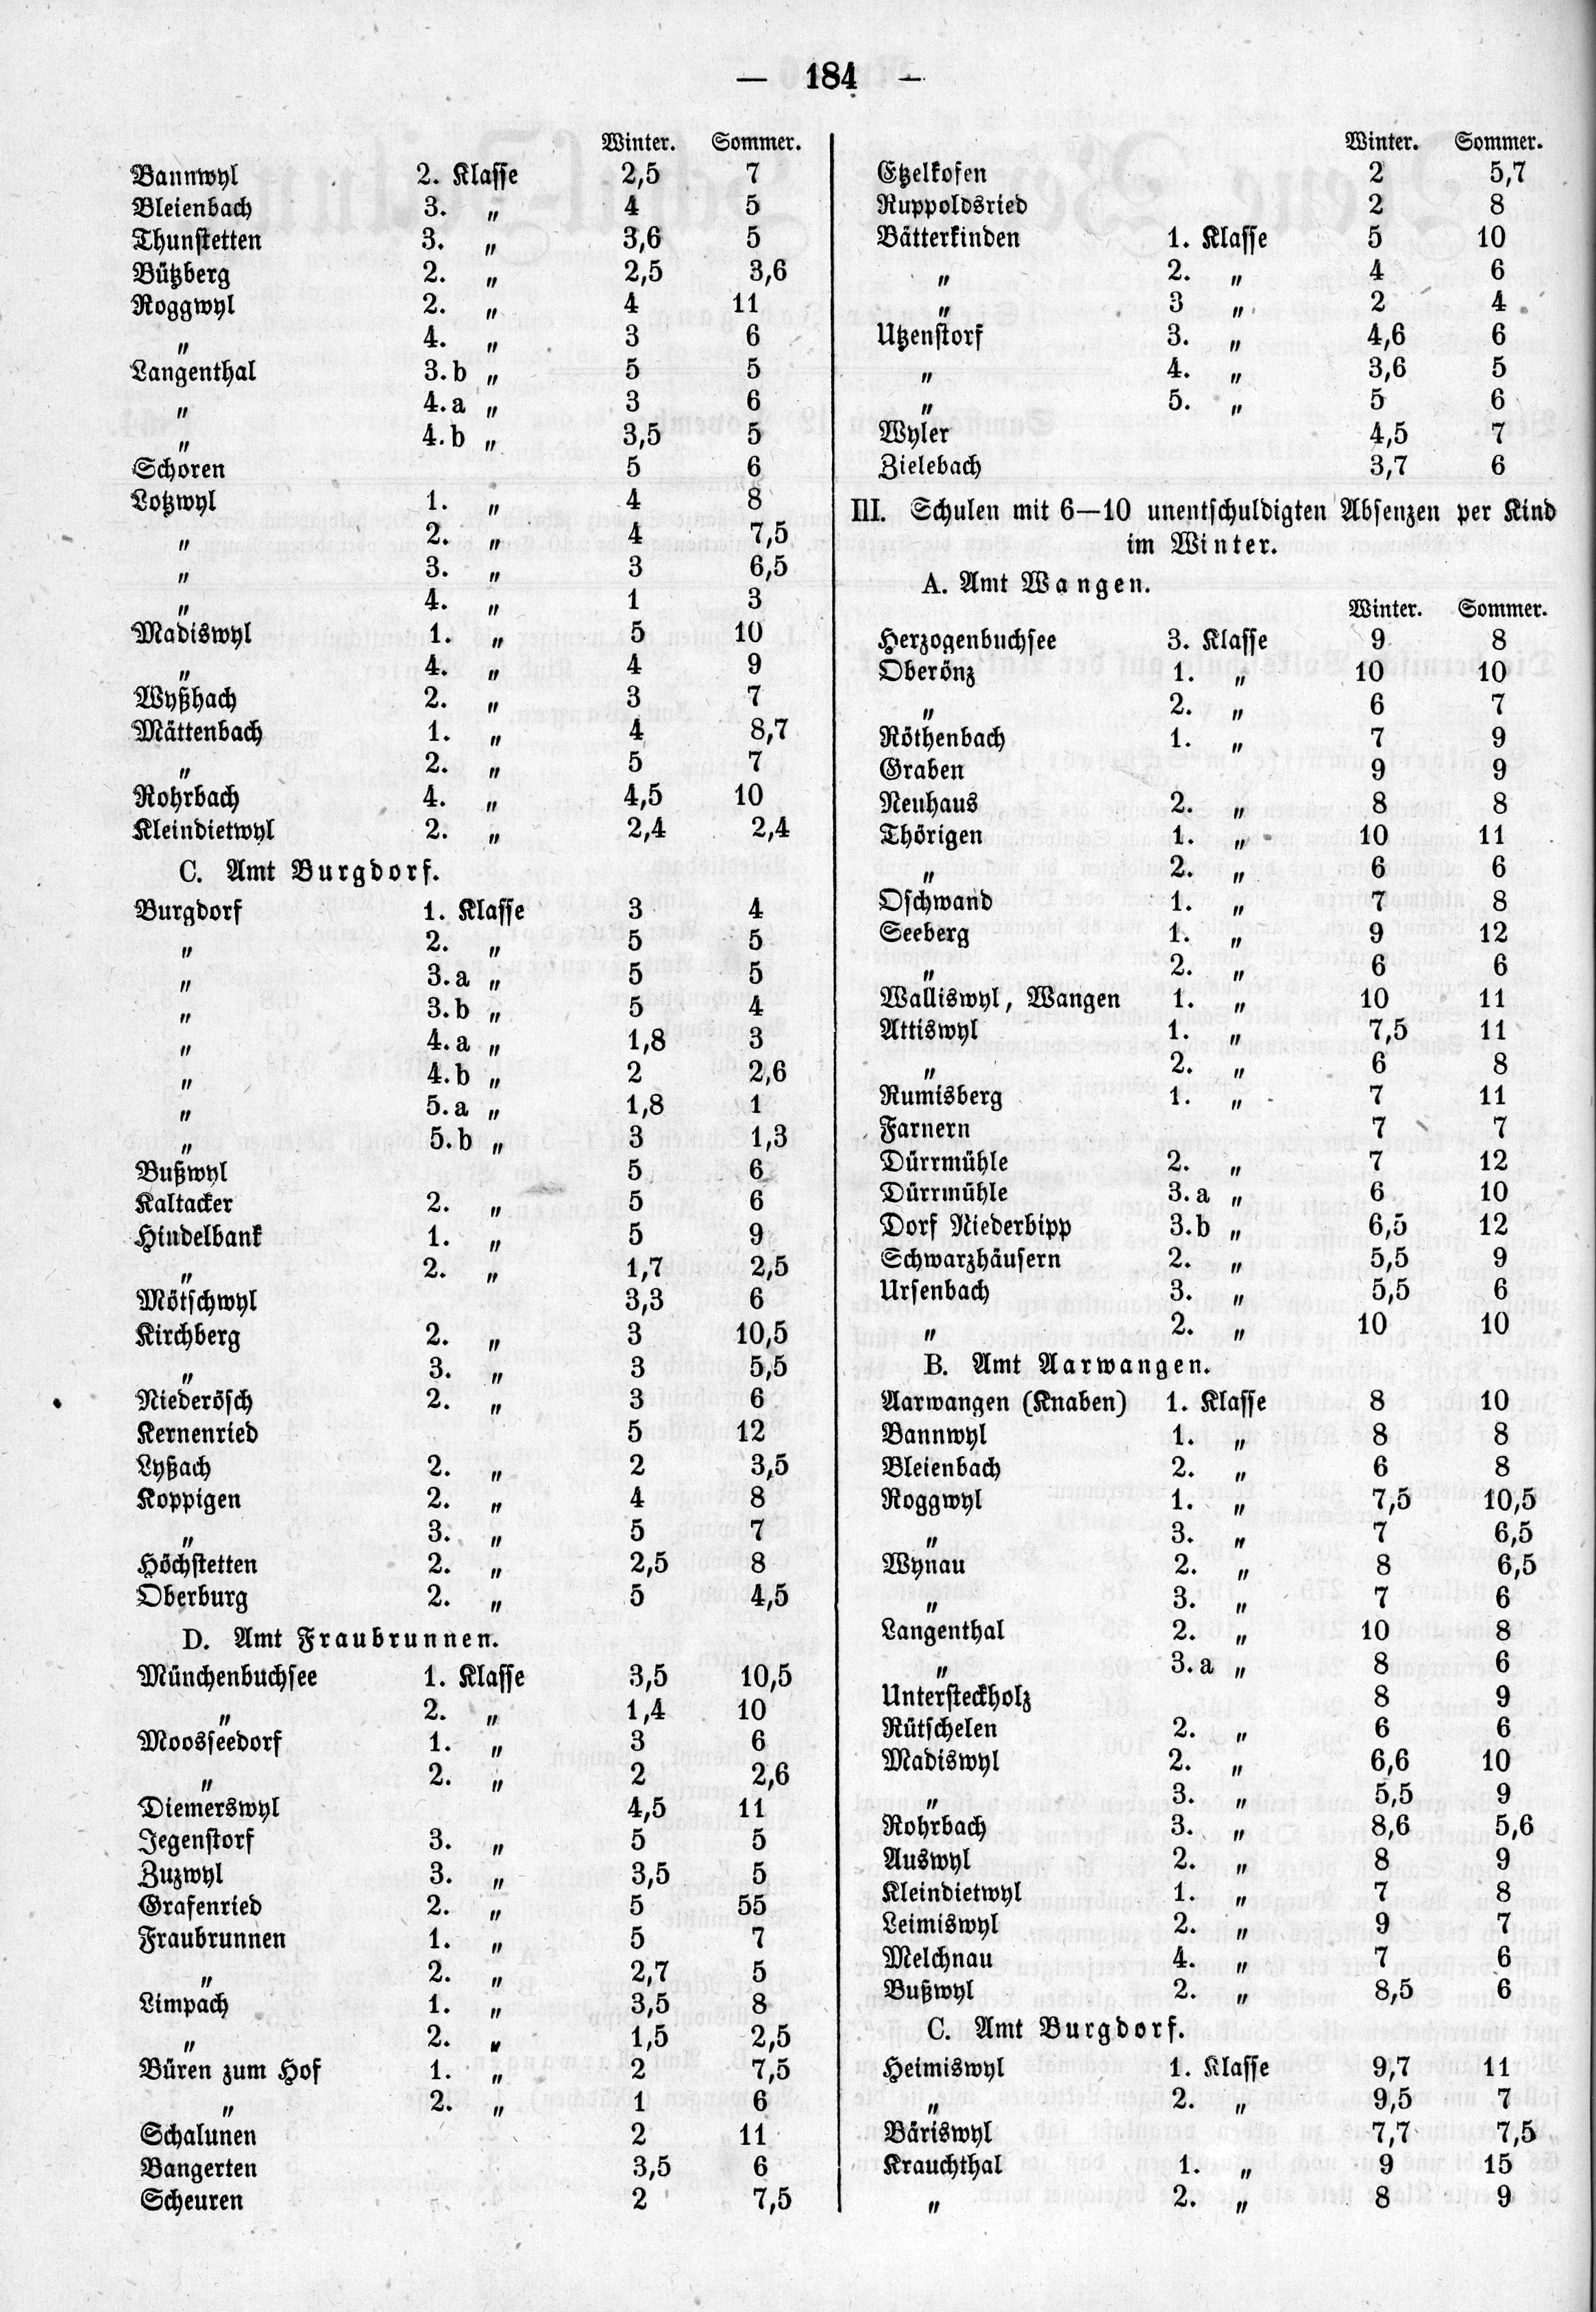
\includegraphics[width=0.8\textwidth]{./Figures/bso-001_1864_007_0184.jpg}
    \caption{Schulabsenzen im Oberaargau 1864 aus~\cite[184]{noauthor_bernische_1864}.}
    \label{figure:5-8}
\end{figure}

\pagebreak

Im Jahr 1864 sorgt ein mehrteiliger Aufsatz in der «Neuen Berner Schul-Zeitung», «Die bernische Volksschule auf der Anklagebank», für einen weiteren deutlichen Peak. Es ist eine bernische Entgegnung auf einen kritischen Artikel in der «Schweizerischen Lehrerzeitung» zum mangelnden Zustand der Schulen im Kanton Bern, der besonders an den vielen Absenzen festgemacht wurde. Herzstück der Replik ist eine umfassende Tabelle der Schulabsenzen im Oberaargau, aufgeteilt nach Ämtern. Angegeben werden die Absenzen der Schüler nach Ort, Klassenstufe und die Zahl der Absenzen. Als signifikantes Muster werden die Unterschiede der Absenzen im Sommer und Winter ausgemacht (Abbildung~\ref{figure:5-8}). 

Wie Abbildung~\ref{figure:5-6} tragen solche Statistiken zum «Nation Building» des Kantons Bern bei, wenn sie die Gemeinde- und Bezirkszugehörigkeiten im Diskurs reifizieren. Allerdings werden keine Bezüge zwischen den Ämtern oder Orten und ihrer Sozialstruktur hergestellt. Höchstens im Subtext lässt sich die Botschaft identifizieren, dass Bern im Vergleich mit dem Kanton Zürich nicht rückständig ist. Auffällig im Vergleich zu Abbildung~\ref{figure:5-6} ist die Darstellungsform, die sich deutlich in Richtung von statistischen Tabellen bewegt. Noch deutlicher wird diese im Beispiel des Kantons Zürich. Sie zeigt auch die fortschreitende Kategorisierung der Absenzen, die nach verantwortbaren Absenzen, etwa durch Krankheit, und strafbare Absenzen eingeteilt werden. Es werden Durchschnitte pro Schüler berechnet und nach Bezirken aufgestellt, was einen Vergleich der Bezirke erlaubt. Warum aber die Absenzenzahlen im Schuljahr 1857/58 in Zürich 15.02, in Winterthur aber nur 9.26 betragen, wird im Begleittext nicht erklärt (Abbildung~\ref{figure:5-9}).

\begin{figure}[!ht]
    \centering
    \includegraphics[width=0.7\textwidth]{./Figures/syn_001_1858_000_22_60_e105_24.jpg}
    \caption{Schulabsenzen im Kanton Zürich 1856–1858 aus~\cite[24]{noauthor_jahresbericht_1858}.}
    \label{figure:5-9}
\end{figure}

Unter den Treffern zu den Absenzen finden sich nun einige, die die Absenzenzahlen mit soziodemografischen Mustern in Verbindung bringen, so etwa ein Bericht des Waadtländer Staatsrates zu den Schulen im Jahr 1856. Für den Bezirk Orbe werden die sozio-ökonomischen Unterschiede zwischen den Orten im Jura und denen der Ebene als Gründe für Unterschiede der Schulabsenzen angeführt: 

\begin{displayquote}
in den Bergen ist er [der Schulbesuch, M.~K.] viel besser als in der Ebene; hier halten die ländlichen Arbeiten die Kinder oft von der Schule ab. Ferner ist der Geschmack am Unterricht in der Ebene weniger entwickelt als in den Bergen; das erklärt zum Theil die häufigern Absenzen in dem Landestheile, welcher am Fuße des Jura liegt (\cite[287]{noauthor_mittheilungen_1858}).
\end{displayquote}

Für den Bezirk Yverdon heisst es an gleicher Stelle: 

\begin{displayquote}
Was den Schulbesuch betrifft, so ist ein merkbarer Unterschied zwischen der Stadt und dem Lande. In der ersteren sind die Absenzen und Disciplinarfälle zahlreicher als in den Landgemeinden durch Schuld der Eltern, welche ihre Kinder unter den kleinlichsten Verwänden zurückhalten und sie durch ihr Beispiel und ihre Reden zur Mißachtung der Lehrer anleiten. In den Dörfern im Gegentheil, und besonders in denjenigen, wo ein gewisser Wohlstand herrscht, bemerkt man am Fleiße und an der Gelehrigkeit der Kinder leicht, daß die Eltern den Werth des Unterrichts und einer guten religiösen Erziehung schätzen. Davon sind auszunehmen die armen Gemeinden, wo die Gewohnheiten der Trunkenheit, des Nichtsthuns, des Bettelns das tägliche Leben vieler Familien geworden sind und auf eine traurige Weise auch die Schuljugend anstecken (\cite[287]{noauthor_mittheilungen_1858}).
\end{displayquote}

Durch die Schulstatistik und besonders die Absenzen wird ein sozio-demografisches Bild des Bezirks gezeichnet. Interessanterweise ist es die Stadt, in der die Rückständigkeit beklagt wird. Dagegen wird die Landbevölkerung als bildungsfleissig dargestellt. Scharf von letzterer ausgenommen werden jedoch die armen Gemeinden. Hier werden Bildungsfleiss und ökonomische Lage verknüpft. Für den Waadtländer Staatsrat scheint es klar zu sein, dass arme Familien auch bildungsferne Familien sind.

Andererseits zeigen die Belege auch die Schwierigkeiten im Umgang mit der Statistik als Überwachunstechnologie. Zahlreich werden nachlässig geführte Listen beklagt oder Lehrer verweisen auf die Kompliziertheit und die Mühen des Ausfüllens der Formulare. Der «avalanche of numbers» erzeugte nicht nur Ordnung erzeugt, sondern auch ein zu viel an Daten. Zudem war auch den Zeitgenossen bewusst, dass hinter den scheinbar eindeutigen Zahlen oft zweifelhafte Erhebungspraktiken standen. Dies ist ebenfalls ein Befund der kritischen Statistikgeschichte (nur ein Beispiel:~\cite[88]{bruckweh_menschen_2015}). Entsprechend finden sich auch im Korpus Belege, die den Wert einer auf Zahlen reduzierten Messung der Schulqualität anzweifeln: 

\begin{displayquote}So wie sich aber diese Kontrolle fast ausschließlich nur auf die Absenztabellen beschränkte, so eben auch der Jahresbericht, und man gab sich so ziemlich dem Glauben hin, als seien die Absenztabellen der sicherste Maßstab zur Beurtheilung des Zustandes der Schulen (\cite[272]{noauthor_schulvisitationen_1855}).
\end{displayquote}

\section{Kontrollüberschuss von Statistiken}
Das Interessante an der Entbergung latenter Muster anhand statistischer Daten ist, dass Daten stets mehr verraten können als den Zweck, für den sie erhoben werden. Dafür sorgt die ihre «radikale Rekombinationsfähigkeit» (\cite[128]{nassehi_muster_2019}). Auf Zahlen reduzierte soziale Phänomene sind frei kombinierbar. Sie können ausserhalb ihres Verwendungskontextes eingesetzt und mit anderen Zahlen in Bezug gesetzt werden: Daten werden verknüpft und neue Einsichten in gesellschaftliche Muster sind im Diskurs formulierbar. Auch dieses Phänomen findet sich im vorliegenden Korpus im Fall von Statistiken. So behandelte ein anonymer Autor in der «Neuen Berner Schulzeitung» 1865 die Frage «Ist die physische Entartung der jetzigen Generation eine Thatsache?» und kombinierte in seiner Problemanalyse medizinische und Schulstatistiken: 

\begin{displayquote}
    Ueber den nachtheiligen Einfluß unzweckmäßiger Einrichtungen geben uns den sichersten Aufschluß die Journale der Aerzte, die Todtenlisten und die Zahl der stets auf betrübende Weise zunehmenden Fälle von Rückgratskrümmungen, Brustkrankheiten, Kopfschmerzen und Augenleiden unserer Schuljugend und unsere daher rührenden Absenzenverzeichnisse (\cite[70]{j_erste_1865}).
\end{displayquote}

Auf sprachlicher Ebene äussert sich dies in diesem Zitat in einer Aufzählung verschiedener Arten von Listen, deren Kombination «Aufschluß gibt», und zwar über die baulichen Zustände der Schulhäuser. Das ist etwas völlig anderes als das, wofür die Absenzenverzeichnisse, Medizinalstatistiken und Mortalitätslisten ursprünglich erstellt worden waren.

Den Statistiken ist also ein «Kontrollüberschuss» (Dirk Baecker, zit.~n.~\cite[43-44]{nassehi_muster_2019}). Durch ihre Rekombinationsfähigkeit enthalten Daten stets ein mehr Informationen, dass sich für Rückschlüsse auf Regelungsbedürftiges nutzen lässt. Ein Beispiel aus dem Korpus ist dafür Treffer 10 in Tabelle~\ref{table:5-2}. Darin kommentiert der Autor den Amtsbericht des evangelischen Erziehungsrats des Kantons St.~Gallen für das Jahr 1855. Die in der Statistik enthaltenen Zahlen werden als Fakten zitiert, denen eine Beweisfunktion zukommt. Auf dieser Grundlage schliesst der Kommentator, die auf tiefgehende Missstände im Umkreis der Schule:

\begin{displayquote}
    «In Starkenbach zeigt die Absenzentabelle auf einen Schüler durchschnittlich 9½, in Wintersberg 12 und in Ennetbühl 17 unentschuldigte Abwesenheiten.» Wo solche Krebsschäden sich zeigen, da suche man die Ursache nicht an einem Orte, und erinnere herzhaft nicht nur die Eltern, sondern auch Lehrer und Schulräthe an ihre Pflichten. Nur radikales Einschreiten kann da helfen, wo Nachläßigkeit und Gleichgültigkeit das Schulleben anzugreifen drohen (\cite{sch_mittheilungen_1856}).
\end{displayquote}

Hier wird von den diskursiv eingeführten Zahlen auf gesellschaftliche Zustände geschlossen. Die Statistik erweist sich nicht nur als Kontrollmittel der Schülerinnen und Schüler sowie ihrer Eltern, sondern auch von Amtspersonen wie den Schulräten. Die Tabellen entdecken nicht nur ein Muster im Absenzverhalten der Schülerinnen, sondern vielmehr Nachlässigkeiten im Disziplinierungsapparat. Sie sind ein Mittel der «Biopolitik». Es wird nicht gemessen, um zu wissen, sondern um andere zu einem erwünschten Verhalten zu disziplinieren. Eine solche datengestützte Form der Disziplinierung ist nur möglich in einer Gesellschaft, die digital sehen gelernt hat, ergo digitalisiert ist (\cite[309-310]{nassehi_muster_2019}).  

\section{Zwischenfazit}
Statistiken im Schweizer Schuldiskurs des 19.~Jahrhunderts zählten Schüler*innen vor allem nach Schulort und Geschlecht. Festgestellt wurde auch eine zunehmend komplexere Kategorisierung, die weitere Kategorien erhob. Allerdings konnte im Korpus weder eine klare Tendenz dahingehend festgestellt werden, dass die Erhebung dieser zusätzlichen Kategorien weiter verbreitet gewesen wäre. Auch Belege zu einer expliziten Kombination der Schüler*innenzahlen wurden kaum gefunden. Was die Statistiken im Diskurs «zeigen», wenn auf sie sprachlich verwiesen wurde, sind meist eben die Zahlen zur Anzahl nach Ort aufgeschlüsselt.

Anhand der Schulabsenzen konnten dagegen Belege gefunden werden, die die Hypothesen dieser Arbeit stützen. Es konnte gezeigt werden, dass die Statistiken und Tabellen eine Überwachungs- und Kontrollfunktion innehatten. Diese erstreckte sich nicht nur auf die Schüler*innen und ihre Eltern, sondern auch auf Lehrer und die Schulgemeinden. 